\documentclass[12pt,a4paper]{report}
\usepackage[utf8]{inputenc}
\usepackage[T1]{fontenc}
\usepackage{amsmath,amssymb,amsfonts}
\usepackage{geometry}
\usepackage{graphicx}
\usepackage{listings}
\usepackage{xcolor}
\usepackage{hyperref}
\usepackage{booktabs}
\usepackage{array}
\usepackage{tikz}
\usepackage{pgfplots}
\pgfplotsset{compat=1.18}
\usetikzlibrary{arrows.meta,shapes,positioning,calc}
\usepackage{subcaption}
\usepackage{float}
\usepackage{parskip}

\geometry{margin=2.5cm}

\hypersetup{
  colorlinks=true,
  linkcolor=blue,
  urlcolor=blue,
  citecolor=blue
}

\lstset{
  basicstyle=\ttfamily\footnotesize,
  keywordstyle=\color{blue}\bfseries,
  commentstyle=\color{gray},
  stringstyle=\color{red!70},
  breaklines=true,
  frame=single,
  backgroundcolor=\color{gray!5},
  numbers=left,
  numberstyle=\tiny\color{gray},
  captionpos=b
}

\title{%
  \textbf{\Large PX4 Fixed-Wing Autosoaring Implementation}\\[1em]
  \large Complete Technical Defence Report\\[0.5em]
  \normalsize Gliding and Thermalling Modes: Architecture, Mathematics, and Implementation\\[2em]
  \textit{Six-Part Report Series}
}
\author{Radhouene --- Fixed-Wing Autosoaring Project}
\date{April 2026}

\begin{document}

\maketitle

\begin{abstract}
This document is a complete technical report of the autosoaring
implementation for a PX4-based fixed-wing UAV, covering engine-off gliding
and thermal soaring. The work modifies six subsystems of the PX4 autopilot:
the uORB/DDS inter-process communication layer, the Total Energy Control
System (TECS), the Fixed-Wing Position Control module, the Commander, the
Navigator, and the ROMFS airframe and parameter definitions.

Each of the six reports below presents: (i) the original system design and
mathematical model, (ii) the motivation for modification, and (iii) the
complete modified design with equations, physics, and code.

This document is intended to prepare the author for a thesis defence by
providing a self-contained, mathematically rigorous reference.
\end{abstract}

\tableofcontents
\listoftables

\newpage

%=============================================================================
% PART I: COMMUNICATIONS
%=============================================================================
\part{Inter-Process Communication and Message Design}

\chapter{uORB Messaging and XRCE-DDS Bridge}

\section{Introduction}

This report describes the inter-process communication (IPC) infrastructure
used to command the autosoaring system from a ROS\,2 companion computer to
the PX4 flight management unit (FMU). It covers:
\begin{itemize}
  \item the uORB publish-subscribe middleware;
  \item the XRCE-DDS bridge connecting ROS\,2 to uORB;
  \item the original messaging approach (boolean flags and a hidden parameter);
  \item the redesigned \texttt{AutosoaringControl} message using a single
        enumerated mode integer;
  \item the \texttt{AutosoaringStatus} message (\texttt{/fmu/out/autosoaring\_status})
        for FMU $\rightarrow$ companion acknowledgement of \texttt{soar:off} and
        the DDS inhibit deadline.
\end{itemize}

\section{Original System: uORB and the Absence of Soaring IPC}

\subsection{uORB Publish-Subscribe Middleware}

PX4 uses \emph{uORB} (micro Object Request Broker) as its internal IPC bus.
It is a strongly-typed, zero-copy, publish-subscribe system running entirely
inside the NuttX RTOS. Each \emph{topic} is defined by a \texttt{.msg} file
and compiled into a C struct with an 8-byte timestamp header.

Key properties:
\begin{itemize}
  \item \textbf{Single writer, multiple readers.}
  \item \textbf{Non-blocking API:} \texttt{orb\_check()} tests for new data;
        \texttt{px4\_poll()} blocks.
  \item \textbf{Fixed-size structs:} no dynamic allocation.
\end{itemize}

\subsection{XRCE-DDS Bridge}

The \texttt{uxrce\_dds\_client} module implements the DDS-XRCE
protocol. Topics listed under \texttt{subscriptions} in
\texttt{dds\_topics.yaml} flow from ROS\,2 into the FMU via
\texttt{/fmu/in/}; topics under \texttt{publications} flow out.

\begin{center}
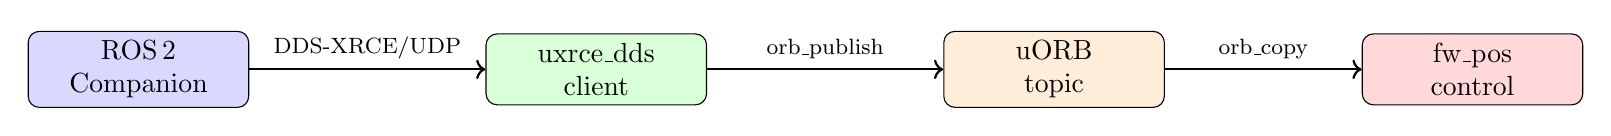
\begin{tikzpicture}[node distance=2.2cm,
    box/.style={draw,rounded corners,minimum width=2.8cm,minimum height=0.8cm,align=center}]
  \node[box,fill=blue!15] (ros) {ROS\,2\\Companion};
  \node[box,fill=green!15,right=3cm of ros] (dds) {uxrce\_dds\\client};
  \node[box,fill=orange!15,right=3cm of dds] (uorb) {uORB\\topic};
  \node[box,fill=red!15,right=2.5cm of uorb] (mod) {fw\_pos\\control};
  \draw[->,thick] (ros) -- node[above]{\footnotesize DDS-XRCE/UDP} (dds);
  \draw[->,thick] (dds) -- node[above]{\footnotesize orb\_publish} (uorb);
  \draw[->,thick] (uorb) -- node[above]{\footnotesize orb\_copy} (mod);
\end{tikzpicture}
\end{center}

In the original \emph{Music} codebase, no soaring topic was registered.

\section{Modified System: AutosoaringControl Message Design}

\subsection{Design Rationale}

The first prototype used two boolean fields: \texttt{glide\_mode\_enabled}
and \texttt{thermal\_mode\_enabled}. This creates four possible combinations,
one of which (both true) is ambiguous. A separate PX4 parameter
\texttt{FW\_GLIDE\_MODE} selected between fixed and polar glide, creating
a hidden third dimension invisible in the message.

The redesign encodes all five states in a single \texttt{uint8 soaring\_mode}:

\begin{center}
\begin{tabular}{clll}
\toprule
Value & Constant & TECS & Navigator \\
\midrule
0 & \texttt{SOARING\_OFF}            & powered        & unchanged \\
1 & \texttt{SOARING\_GLIDE\_FIXED}   & gliding, fixed EAS & AUTO\_MISSION \\
2 & \texttt{SOARING\_GLIDE\_POLAR}   & gliding, polar EAS & AUTO\_MISSION \\
3 & \texttt{SOARING\_THERMAL\_LOITER}& gliding        & AUTO\_LOITER (navigator) \\
4 & \texttt{SOARING\_THERMAL\_BANK}  & gliding        & AUTO\_LOITER (roll override) \\
\bottomrule
\end{tabular}
\end{center}

\subsection{Complete AutosoaringControl Message}

\begin{lstlisting}[language=,caption={msg/AutosoaringControl.msg (new file)}]
uint64  timestamp               # microseconds since boot

uint8   soaring_mode            # active mode
uint8 SOARING_OFF             = 0
uint8 SOARING_GLIDE_FIXED     = 1
uint8 SOARING_GLIDE_POLAR     = 2
uint8 SOARING_THERMAL_LOITER  = 3
uint8 SOARING_THERMAL_BANK    = 4

# Loiter geometry (mode 3 only)
float32 loiter_radius_m         # [m]; NaN => bank-derived minimum
float32 loiter_lat              # [deg]; NaN/0 => current position
float32 loiter_lon              # [deg]; NaN/0 => current position

# Optimisation (NaN => PX4 default)
float32 airspeed_cmd            # [m/s EAS]  mode 1 only
float32 bank_angle_cmd          # [deg]       modes 3,4
bool    loiter_clockwise        # true=CW, false=CCW

# Metadata
uint8   soaring_phase           # companion-reported phase
uint8 SOARING_PHASE_CRUISE    = 0
uint8 SOARING_PHASE_GLIDING   = 1
uint8 SOARING_PHASE_SEARCHING = 2
uint8 SOARING_PHASE_CENTERING = 3
uint8 SOARING_PHASE_THERMAL   = 4
\end{lstlisting}

\subsection{Field Usage Matrix}

\begin{center}
\begin{tabular}{lccccc}
\toprule
Field & Mode 0 & Mode 1 & Mode 2 & Mode 3 & Mode 4 \\
\midrule
\texttt{airspeed\_cmd}     & -- & \checkmark & -- & -- & -- \\
\texttt{loiter\_radius\_m} & -- & -- & -- & \checkmark & -- \\
\texttt{loiter\_lat/lon}   & -- & -- & -- & \checkmark & -- \\
\texttt{bank\_angle\_cmd}  & -- & -- & -- & \checkmark & \checkmark \\
\texttt{loiter\_clockwise} & -- & -- & -- & \checkmark & \checkmark \\
\bottomrule
\end{tabular}
\end{center}

\subsection{AutosoaringStatus (FMU $\rightarrow$ companion)}

\texttt{msg/AutosoaringStatus.msg} is published by \texttt{fw\_pos\_control} and
bridged out as \texttt{/fmu/out/autosoaring\_status}. Fields include
\texttt{source} (\texttt{SOURCE\_CLI\_SOARING\_OFF} or
\texttt{SOURCE\_STALENESS\_WATCHDOG}), \texttt{soaring\_mode\_effective}, and
\texttt{dds\_inhibit\_until\_us} (absolute time until DDS ``soaring on'' is
accepted again; zero if none). While the post-\texttt{soar:off} inhibit is
active, status is republished at 1\,Hz.

\begin{lstlisting}[language=,caption={dds\_topics.yaml (publications excerpt)}]
  - topic: /fmu/out/autosoaring_status
    type: px4_msgs::msg::AutosoaringStatus
\end{lstlisting}

\subsection{Staleness Watchdog}

If the companion is silent for more than 2\,s while a soaring mode is
active:
\begin{equation}
  \Delta t_{\text{silence}} > 2\,\text{s}
  \quad\Rightarrow\quad
  \texttt{soaring\_mode} \leftarrow 0
\end{equation}

The FMU also publishes \texttt{AutosoaringStatus} with
\texttt{SOURCE\_STALENESS\_WATCHDOG}. This prevents the aircraft from remaining
in engine-off glide indefinitely if the companion crashes or the DDS link fails.

\subsection{Summary}

\begin{center}
\begin{tabular}{p{3.5cm}p{4.5cm}p{4.5cm}}
\toprule
Aspect & Original & Modified \\
\midrule
Mode encoding & Two booleans + hidden param & Single \texttt{uint8 soaring\_mode} \\
DDS in (commands) & Not present & \texttt{/fmu/in/autosoaring\_control} \\
DDS out (status) & Not present & \texttt{/fmu/out/autosoaring\_status} \\
Turn direction & Not supported & \texttt{loiter\_clockwise} bool \\
Staleness guard & Not present & 2\,s watchdog + status publish \\
\bottomrule
\end{tabular}
\end{center}

%=============================================================================
% PART II: TECS
%=============================================================================
\part{Total Energy Control System}

\chapter{TECS: Original Architecture and Soaring Extensions}

\section{Introduction}

TECS (Total Energy Control System) is the primary flight envelope controller
for fixed-wing aircraft in PX4, originally proposed by Lambregts (1983).
It controls airspeed and altitude simultaneously through two decoupled
channels: throttle controls the total specific energy, and pitch controls
the energy balance.

\section{Original TECS: Mathematical Foundation}

\subsection{Specific Energy Definitions}

Let $m$ be the aircraft mass, $g$ gravitational acceleration, $V$ the true
airspeed, and $h$ the altitude. The specific (per unit weight) energies are:
\begin{align}
  E_k &= \frac{V^2}{2g} \quad [\text{m}]
         \quad\text{(specific kinetic energy)} \\
  E_p &= h \quad [\text{m}]
         \quad\text{(specific potential energy)} \\
  E   &= E_k + E_p = \frac{V^2}{2g} + h \quad [\text{m}]
\end{align}

Their time derivatives (specific energy rates):
\begin{align}
  \dot{E}_k &= \frac{V\dot{V}}{g} \\
  \dot{E}_p &= \dot{h} \\
  \dot{E}   &= \frac{V\dot{V}}{g} + \dot{h}
\end{align}

\subsection{Throttle Control Law}

The STE rate setpoint is:
\begin{equation}
  \dot{E}^* = \dot{E}_k^* + \dot{E}_p^*
            + K_{\text{lf}}(n_z - 1)
\end{equation}

where $n_z = 1/\cos\phi$ is the load factor and $K_{\text{lf}}$ is the
load-factor correction gain. The throttle demand:
\begin{equation}
  \delta_t = \frac{\dot{E}^* - \hat{\dot{E}}}{c_1}\,K_{\text{damp}}
           + \delta_{t,\text{pred}} + I_t
\end{equation}

The integrator:
\begin{equation}
  \dot{I}_t = K_{i,t}(\dot{E}^* - \hat{\dot{E}})
\end{equation}

\subsection{Pitch Control Law}

Energy balance rate setpoint:
\begin{equation}
  \dot{B}^* = w_{\text{ske}}\,\dot{E}_k^* - w_{\text{spe}}\,\dot{E}_p^*
\end{equation}

Pitch angle setpoint:
\begin{equation}
  \theta^* = \frac{1}{V}\!\left[
    K_\theta(\dot{B}^* - \hat{\dot{B}}) + K_d\ddot{B} + I_\theta + \theta_{\text{ff}}
  \right]
\end{equation}

Pitch integrator:
\begin{equation}
  \dot{I}_\theta = K_{i,\theta}(\dot{B}^* - \hat{\dot{B}})
\end{equation}

\subsection{Airspeed Setpoint Computation}

EAS to TAS conversion:
\begin{equation}
  k_{\text{EAS2TAS}} = \sqrt{\frac{\rho_0}{\rho}}, \quad \rho_0 = 1.225\,\text{kg/m}^3
\end{equation}

Powered-flight TAS setpoint:
\begin{equation}
  V_{\text{TAS}}^* = \text{lerp}\!\left(
    k_{\text{EAS2TAS}} V_{\text{EAS}}^*,\;
    V_{\text{TAS,max}},\;
    \alpha_{\text{fd}}
  \right)
\end{equation}

\subsection{Energy Weighting}

The speed weight $w_{\text{ske}} \in [0,2]$ (parameter \texttt{FW\_T\_SPDWEIGHT})
adjusts channel priority. $w_{\text{spe}} = 2 - w_{\text{ske}}$.

\subsection{Underspeed Detection}

\begin{equation}
  r_u = \frac{V_{\text{TAS,min}} - V_{\text{TAS}}}{V_{\text{TAS,min}}\,\varepsilon}
\end{equation}

When $r_u > 0$:
\begin{equation}
  \delta_t \leftarrow r_u\,\delta_{t,\max} + (1-r_u)\,\delta_t
\end{equation}

\section{Modified TECS: Soaring-Mode Extensions}

\subsection{Throttle Integrator Decay During Glide}

To prevent throttle surge on glide exit, the integrator decays:
\begin{equation}
  \boxed{I_t(t) = I_t(0)\,e^{-t/\tau}}
\end{equation}

Discrete-time update ($\alpha_\tau = e^{-\Delta t/\tau}$):
\begin{equation}
  I_t[k+1] = \alpha_\tau\,I_t[k]
\end{equation}

For $\tau = 10\,\text{s}$, $\Delta t = 20\,\text{ms}$:
$\alpha_\tau = e^{-0.002} \approx 0.9980$.

\subsection{Energy Weighting Override in Glide}

Since throttle is zero, all energy management is through pitch:
\begin{equation}
  \boxed{w_{\text{spe}} = 0, \quad w_{\text{ske}} = 2}
\end{equation}

The energy balance becomes:
\begin{equation}
  \dot{B} = 2\,\frac{V\dot{V}}{g}
\end{equation}

\subsection{Glide Polar and Best-Glide Speed (Mode 2)}

Parabolic glide polar:
\begin{equation}
  w_s(V) = aV^2 + b
\end{equation}

Best-glide EAS (maximises range $= V/w_s$):
\begin{equation}
  \boxed{V^*_{\text{EAS,polar}} = \sqrt{\frac{b}{a}}}
\end{equation}

Maximum glide ratio:
\begin{equation}
  \left(\frac{L}{D}\right)_{\max} = \frac{1}{2\sqrt{ab}}
\end{equation}

\subsection{Banked Stall Speed Floor (Thermalling)}

Load factor at bank angle $\phi$:
\begin{equation}
  n_z = \frac{1}{\cos\phi}
\end{equation}

Banked stall speed:
\begin{equation}
  V_{\text{stall,banked}} = V_{\text{stall,level}}\,\sqrt{n_z}
\end{equation}

TECS stall floor:
\begin{equation}
  \boxed{V_{\text{TAS,banked,min}} = V_{\text{TAS,min}}\,\sqrt{n_z}}
\end{equation}

Airspeed setpoint with floor:
\begin{equation}
  V_{\text{TAS}}^* = \max\!\left(
    \text{clamp}(k_{\text{EAS2TAS}}\,V_{\text{EAS}}^*,\;
      V_{\text{TAS,min}},\;V_{\text{TAS,max}}),\;
    V_{\text{TAS,banked,min}}
  \right)
\end{equation}

\textbf{Example} ($\phi = 40^\circ$, $V_{\text{TAS,min}} = 9\,\text{m/s}$):
\begin{align}
  n_z &= 1/\cos 40^\circ = 1.305 \\
  V_{\text{TAS,banked,min}} &= 9\,\sqrt{1.305} \approx 10.3\,\text{m/s}
\end{align}

\subsection{Underspeed Detection Bypass}

In glide, the throttle is forced to zero regardless; the underspeed boost
is meaningless and pollutes telemetry. Fix:
\begin{lstlisting}[language=C++]
if (flag.gliding_mode_enabled) {
    _ratio_undersped = 0.0f;
    return;
}
\end{lstlisting}

\subsection{Load-Factor STE Correction Disabled in Glide}

In powered turns, the STE correction compensates for induced drag:
\begin{equation}
  \dot{E}^* \mathrel{+}= K_{\text{lf}}\,(n_z - 1)
\end{equation}

In glide, throttle is already clamped to zero. The correction is skipped:
\begin{lstlisting}[language=C++]
if (!flag.gliding_mode_enabled) {
    ste_rate.setpoint += param.load_factor_correction * (param.load_factor - 1.f);
}
\end{lstlisting}

\subsection{Pitch Integrator Partial Reset on Entry and Exit}

\subsubsection{Physical Motivation}

On glide \textbf{entry}: $I_\theta$ holds a powered cruise bias. When
$w_{\text{spe}} \leftarrow 0$, this bias commands nose-up, fighting the
speed-hold objective.

On glide \textbf{exit}: $I_\theta$ holds a speed-hold bias. Power restoration
rapidly adds STE; TECS corrects at maximum pitch rate:
\begin{equation}
  \dot{\theta}_{\max} = \frac{a_{z,\text{lim}}}{V}
  \approx \frac{7\,\text{m/s}^2}{10\,\text{m/s}} = 0.7\,\text{rad/s}
  \approx 40\text{--}50\,\text{deg/s}
\end{equation}

\subsubsection{Fix}

Halve the integrator at both transitions:
\begin{equation}
  \boxed{I_\theta \leftarrow \tfrac{1}{2}\,I_\theta}
\end{equation}

\begin{lstlisting}[language=C++]
if (flag.gliding_mode_enabled && !_prev_gliding_mode) {
    _pitch_integ_state *= 0.5f;   // glide entry
} else if (!flag.gliding_mode_enabled && _prev_gliding_mode) {
    _pitch_integ_state *= 0.5f;   // glide exit
}
_prev_gliding_mode = flag.gliding_mode_enabled;
\end{lstlisting}

\subsection{Summary of TECS Modifications}

\begin{center}
\begin{tabular}{p{4cm}p{4.5cm}p{4.5cm}}
\toprule
Behaviour & Original & Modified \\
\midrule
Throttle (unpowered) & Integrator uncontrolled & Hard-zero + $I_t$ decay \\
Pitch weighting & From parameter & $w_{\text{spe}}=0$, $w_{\text{ske}}=2$ \\
Airspeed setpoint & Mission EAS & Fixed (mode 1) or polar (mode 2) \\
Stall floor & $V_{\text{TAS,min}}$ & $V_{\text{TAS,min}}\sqrt{n_z}$ \\
Underspeed & Cruise trim threshold & Bypassed in glide \\
LF correction & Always & Disabled in glide \\
Integrator transitions & No reset & $\times 0.5$ on entry and exit \\
\bottomrule
\end{tabular}
\end{center}

%=============================================================================
% PART III: FW POS CONTROL
%=============================================================================
\part{Fixed-Wing Position Control}

\chapter{FixedwingPositionControl: Soaring Dispatch and Guidance}

\section{Original Architecture}

\subsection{Module Role}

\texttt{FixedwingPositionControl} runs at $\sim 50$\,Hz and:
\begin{enumerate}
  \item reads estimates and the navigator setpoint triplet;
  \item calls NPFG to compute roll (or reads loiter centre from navigator);
  \item calls TECS via \texttt{tecs\_update\_pitch\_throttle};
  \item publishes the attitude setpoint.
\end{enumerate}

\subsection{NPFG Guidance}

Track-error angle $\eta$ from velocity to path tangent drives lateral
acceleration:
\begin{equation}
  a_{\text{lat}} = \frac{2V_a^2}{L}\sin\eta
\end{equation}
Roll setpoint:
\begin{equation}
  \phi^* = \arctan\!\left(\frac{a_{\text{lat}}}{g}\right)
\end{equation}

\subsection{adapt\_airspeed\_setpoint}

Floor-clamped EAS setpoint accounting for load factor:
\begin{equation}
  V_{\text{EAS}}^* = \text{clamp}\!\left(
    V_{\text{sp}},\;
    V_{\text{stall}}\sqrt{n_z},\;
    V_{\text{EAS,max}}
  \right)
\end{equation}

\section{Soaring Mode Dispatch Logic}

\subsection{Mode Derivation}

Each cycle in \texttt{control\_auto()}:
\begin{lstlisting}[language=C++]
const bool glide_cmd   = (soaring_cmd == SOARING_GLIDE_FIXED
                       || soaring_cmd == SOARING_GLIDE_POLAR);
const bool thermal_cmd = (soaring_cmd == SOARING_THERMAL_LOITER
                       || soaring_cmd == SOARING_THERMAL_BANK);
const bool soaring_allowed = (soaring_cmd != SOARING_OFF)
    && (_current_altitude > _param_fw_alt_min.get()
        || _soaring_local_override);
const bool effective_glide = soaring_allowed
    && (glide_cmd || _alt_max_reached);
const bool effective_thermal = soaring_allowed && thermal_cmd
    && !_alt_max_reached;
const bool effective_thermal_bank = effective_thermal
    && (soaring_cmd == SOARING_THERMAL_BANK);
\end{lstlisting}

\subsection{Altitude Ceiling and Floor}

Floor check:
\begin{equation}
  h < h_{\min} \;\Rightarrow\; \texttt{soaring\_allowed} = \text{false}
\end{equation}

Ceiling:
\begin{equation}
  h \geq h_{\max} \;\Rightarrow\; \texttt{\_alt\_max\_reached} = \text{true}
\end{equation}
\begin{equation}
  h < h_{\max} - h_{\text{hyst}} \;\Rightarrow\; \texttt{\_alt\_max\_reached} = \text{false}
\end{equation}

\section{Throttle Ramps}

\subsection{Entry Ramp (Powered $\rightarrow$ Glide)}

\begin{equation}
  \delta_t(t) = \delta_{t,\text{pre}}\left(1 - \frac{t - t_s}{T_{\text{ramp}}}\right), \quad t \in [t_s,\; t_s + T_{\text{ramp}}]
\end{equation}

\subsection{Exit Ramp (Glide $\rightarrow$ Powered)}

\begin{equation}
  \delta_t(t) = \delta_{t,\text{TECS}}\,\frac{t - t_e}{T_{\text{ramp}}}, \quad t \in [t_e,\; t_e + T_{\text{ramp}}]
\end{equation}

Both ramps use $T_{\text{ramp}}$ = \texttt{FW\_GLIDE\_RAMP\_T}.

\section{Airspeed Setpoints per Mode}

\begin{center}
\begin{tabular}{clp{7cm}}
\toprule
Mode & Airspeed & Computation \\
\midrule
1 & Fixed & $V^* = \texttt{FW\_GLIDE\_AIRSPD}$ (or \texttt{airspeed\_cmd}) \\
2 & Polar & $V^* = \sqrt{b/a}$, computed per cycle \\
3,4 & Hold & $V^* = \texttt{FW\_GLIDE\_AIRSPD}$ \\
\bottomrule
\end{tabular}
\end{center}

\section{Mode 3: Thermal Loiter via Navigator}

\subsection{Loiter Radius}

Minimum safe radius at bank $\phi$, speed $V_{\text{TAS}}$:
\begin{equation}
  R_{\min} = \frac{V_{\text{TAS}}^2}{g\tan\phi}
\end{equation}

Effective radius:
\begin{equation}
  R_{\text{eff}} = \max(R_c,\; R_{\min})
\end{equation}

\subsection{Signed Radius Encoding}

\begin{equation}
  \texttt{param3} = \begin{cases}
    +R_{\text{eff}} & \text{clockwise} \\
    -R_{\text{eff}} & \text{counter-clockwise}
  \end{cases}
\end{equation}

\subsection{Pre-Roll Safety (T3)}

Before first DO\_REPOSITION:
\begin{equation}
  V_{\text{EAS,current}} \geq 1.05\,V_{\text{stall}}\sqrt{n_z}
\end{equation}

If not satisfied, the command is delayed until speed is sufficient.

\section{Mode 4: Direct Bank-Angle Thermal Guidance}

\subsection{Why Bypass NPFG}

Mode 4 bypasses the \texttt{switch(position\_sp\_type)} block entirely.
Calling NPFG first would contaminate TECS with loiter-geometry-adjusted
airspeed. By calling TECS directly and composing the quaternion manually,
both pitch and roll are under explicit control.

\subsection{Roll Sign Convention}

\begin{equation}
  \phi^* = s\,|\phi_{\text{cmd}}|, \quad
  s = \begin{cases}
    +1 & \texttt{loiter\_clockwise} = \text{true} \\
    -1 & \texttt{loiter\_clockwise} = \text{false}
  \end{cases}
\end{equation}

\subsection{Attitude Setpoint Composition}

\begin{equation}
  \mathbf{q}^* = \text{Euler}(\phi^*,\,\theta_{\text{TECS}},\,\psi_{\text{current}})
\end{equation}

\begin{lstlisting}[language=C++]
const float bank_rad = bank_sign * math::radians(fabsf(_soaring_bank_angle_cmd_deg));
const Quatf q_bank(Eulerf(bank_rad, get_tecs_pitch(), _yaw));
q_bank.copyTo(_att_sp.q_d);
_att_sp.thrust_body[0] = get_tecs_thrust();
\end{lstlisting}

\subsection{Summary}

\begin{center}
\begin{tabular}{p{4cm}p{4.5cm}p{4.5cm}}
\toprule
Feature & Original & Modified \\
\midrule
Mode encoding & Two booleans & Single integer \\
Entry ramp & Instant cut & Smooth ($T_{\text{ramp}}$) \\
Exit ramp & Instant & Smooth ($T_{\text{ramp}}$) \\
Mode 4 roll & Not present & Direct bank-angle \\
Turn direction & Not supported & Signed radius + bool \\
Pre-roll safety & Not present & Banked stall check \\
\bottomrule
\end{tabular}
\end{center}

%=============================================================================
% PART IV: COMMANDER
%=============================================================================
\part{Commander: CLI Mode Switching}

\chapter{Commander Soaring Commands}

\section{Original System}

In the original Music codebase, Commander had no soaring-specific CLI
commands. Soaring behaviour required manual parameter changes via a GCS.

\section{Modified System: CLI Commands}

\subsection{Commands Added}

\begin{lstlisting}[language=bash]
commander mode soar:off      # mode 0 -- powered flight
commander mode soar:glide    # mode 1 -- fixed-EAS glide
commander mode soar:polar    # mode 2 -- polar best-glide
commander mode soar:thermal  # mode 3 -- navigator loiter
commander mode soar:bank     # mode 4 -- direct bank angle
\end{lstlisting}

\subsection{Command Structure}

Each command publishes \texttt{VEHICLE\_CMD\_CUSTOM\_0} with
\texttt{param1 = (float)soaring\_mode}.

\subsection{Local-Override Flag}

CLI commands set \texttt{\_soaring\_local\_override = true}, which:
\begin{itemize}
  \item bypasses altitude floor check;
  \item disables staleness watchdog;
  \item is cleared on disarm or explicit \texttt{soar:off}.
\end{itemize}

%=============================================================================
% PART V: NAVIGATOR
%=============================================================================
\part{Navigator: Loiter Direction Control}

\chapter{Navigator DO\_REPOSITION Extension}

\section{Original Handler}

\begin{lstlisting}[language=C++,caption={Original -- positive radius only}]
if (PX4_ISFINITE(cmd.param3) && cmd.param3 > 0) {
    rep->current.loiter_radius = cmd.param3;
    // direction never set from param3
}
\end{lstlisting}

\section{Modified Handler}

\begin{lstlisting}[language=C++,caption={Modified -- signed radius encodes direction}]
if (PX4_ISFINITE(cmd.param3) && fabsf(cmd.param3) > FLT_EPSILON) {
    rep->current.loiter_radius = fabsf(cmd.param3);
    rep->current.loiter_direction_counter_clockwise = (cmd.param3 < 0.f);
}
\end{lstlisting}

\subsection{Circular Flight Mathematics}

Angular rate:
\begin{equation}
  \omega = \frac{V_{\text{TAS}}}{R}
\end{equation}

Turn direction:
\begin{equation}
  \omega = \begin{cases}
    +|V/R| & \text{CCW (NED)} \\
    -|V/R| & \text{CW (NED)}
  \end{cases}
\end{equation}

Encoding:
\begin{equation}
  \texttt{loiter\_direction\_counter\_clockwise} = (\texttt{param3} < 0)
\end{equation}

\section{Direction-Change Trigger}

A new \texttt{direction\_changed} flag forces resend when only
\texttt{loiter\_clockwise} changes:
\begin{lstlisting}[language=C++]
const bool direction_changed =
    (_autosoaring_control.loiter_clockwise != _soaring_last_clockwise);
const bool pos_changed = (first_activation && ok) || explicit_pos_changed
    || direction_changed;
\end{lstlisting}

After sending, \texttt{\_soaring\_last\_clockwise} is latched to prevent
repeated re-sends.

%=============================================================================
% PART VI: ROMFS AND PARAMETERS
%=============================================================================
\part{ROMFS and Parameter Definitions}

\chapter{Soaring Parameters and Airframe Configuration}

\section{Parameter System Overview}

PX4 parameters are compiled into flash with defaults via
\texttt{PARAM\_DEFINE\_*} macros. The ROMFS airframe script overrides
defaults for a specific vehicle.

\section{Removed Parameter: FW\_GLIDE\_MODE}

The parameter \texttt{FW\_GLIDE\_MODE} (integer, 0=fixed, 1=polar) was
removed. Its function is now encoded in \texttt{soaring\_mode} = 1 or 2.

\section{New Parameters}

\subsection{FW\_GLIDE\_AIRSPD (10.0 m/s EAS)}

Fixed glide airspeed and thermalling reference speed.
\begin{equation}
  V_{\text{TAS}}^* = \sqrt{\frac{\rho_0}{\rho}}\,\times\,10.0\,\text{m/s}
\end{equation}

\subsection{FW\_POLAR\_A (0.003 s/m) and FW\_POLAR\_B (0.5 m/s)}

Parabolic polar: $w_s = aV^2 + b$.

Best-glide speed:
\begin{equation}
  V^*_{\text{polar}} = \sqrt{0.5/0.003} \approx 12.9\,\text{m/s}
\end{equation}

Maximum glide ratio:
\begin{equation}
  (L/D)_{\max} = 1/(2\sqrt{0.003\times 0.5}) \approx 12.9
\end{equation}

\subsection{FW\_GLIDE\_I\_DECAY (10.0 s)}

Throttle integrator decay constant:
\begin{equation}
  I_t(t) = I_t(0)\,e^{-t/10} \quad\Rightarrow\quad
  I_t(30\,\text{s}) = I_t(0)\,e^{-3} \approx 0.05\,I_t(0)
\end{equation}

\subsection{FW\_GLIDE\_RAMP\_T (3.0 s)}

Throttle ramp duration. At 50\,Hz: 150 cycles. Rate: $\delta_t(0)/T = 0.133/\text{s}$.

\subsection{FW\_THERMAL\_BANK (40 deg)}

Default bank angle. Load factor and minimum radius:
\begin{align}
  n_z &= 1/\cos 40^\circ = 1.305 \\
  R_{\min} &= \frac{V^2}{g\tan 40^\circ}
            = \frac{10^2}{9.81 \times 0.839} \approx 12.2\,\text{m}
\end{align}

\subsection{FW\_ALT\_MIN (50 m), FW\_ALT\_MAX (200 m), FW\_ALT\_HYST (20 m)}

Soaring altitude envelope with ceiling hysteresis.

\section{ROMFS Airframe Defaults}

Added to \texttt{ROMFS/px4fmu\_common/init.d/airframes/4008\_gz\_advanced\_plane}:

\begin{lstlisting}[language=bash]
param set FW_GLIDE_AIRSPD   10.0
param set FW_POLAR_A         0.003
param set FW_POLAR_B         0.5
param set FW_GLIDE_I_DECAY  10.0
param set FW_GLIDE_RAMP_T    3.0
param set FW_THERMAL_BANK   40.0
param set FW_ALT_MIN        50.0
param set FW_ALT_MAX       200.0
param set FW_ALT_HYST       20.0
\end{lstlisting}

\section{Summary}

\begin{center}
\begin{tabular}{p{4.5cm}p{4cm}p{4.5cm}}
\toprule
Aspect & Original & Modified \\
\midrule
Soaring parameters & None & 9 new parameters \\
FW\_GLIDE\_MODE & Defined & Removed \\
Airframe defaults & None & Added to 4008 airframe \\
\bottomrule
\end{tabular}
\end{center}

%=============================================================================
\appendix
\chapter{ROS 2 Command Reference}
%=============================================================================

\begin{lstlisting}[language=bash,caption={ROS 2 test commands for each soaring mode}]
# Mode 0: OFF (powered)
ros2 topic pub --once /fmu/in/autosoaring_control \
  px4_msgs/msg/AutosoaringControl \
  "{timestamp: 0, soaring_mode: 0, loiter_radius_m: 0.0, loiter_lat: 0.0,
    loiter_lon: 0.0, airspeed_cmd: 0.0, bank_angle_cmd: 0.0,
    loiter_clockwise: true, soaring_phase: 0}"

# Mode 1: Fixed-EAS Glide at 10 m/s
ros2 topic pub --once /fmu/in/autosoaring_control \
  px4_msgs/msg/AutosoaringControl \
  "{timestamp: 0, soaring_mode: 1, loiter_radius_m: 0.0, loiter_lat: 0.0,
    loiter_lon: 0.0, airspeed_cmd: 10.0, bank_angle_cmd: 0.0,
    loiter_clockwise: true, soaring_phase: 1}"

# Mode 2: Polar best-glide
ros2 topic pub --once /fmu/in/autosoaring_control \
  px4_msgs/msg/AutosoaringControl \
  "{timestamp: 0, soaring_mode: 2, loiter_radius_m: 0.0, loiter_lat: 0.0,
    loiter_lon: 0.0, airspeed_cmd: 0.0, bank_angle_cmd: 0.0,
    loiter_clockwise: true, soaring_phase: 1}"

# Mode 3: Thermal loiter, CW, 40-deg bank, R=15m
ros2 topic pub --once /fmu/in/autosoaring_control \
  px4_msgs/msg/AutosoaringControl \
  "{timestamp: 0, soaring_mode: 3, loiter_radius_m: 15.0, loiter_lat: 0.0,
    loiter_lon: 0.0, airspeed_cmd: 0.0, bank_angle_cmd: 40.0,
    loiter_clockwise: true, soaring_phase: 2}"

# Mode 3: Thermal loiter, CCW
ros2 topic pub --once /fmu/in/autosoaring_control \
  px4_msgs/msg/AutosoaringControl \
  "{timestamp: 0, soaring_mode: 3, loiter_radius_m: 15.0, loiter_lat: 0.0,
    loiter_lon: 0.0, airspeed_cmd: 0.0, bank_angle_cmd: 40.0,
    loiter_clockwise: false, soaring_phase: 2}"

# Mode 4: Direct bank angle, 40-deg, CW
ros2 topic pub --once /fmu/in/autosoaring_control \
  px4_msgs/msg/AutosoaringControl \
  "{timestamp: 0, soaring_mode: 4, loiter_radius_m: 0.0, loiter_lat: 0.0,
    loiter_lon: 0.0, airspeed_cmd: 0.0, bank_angle_cmd: 40.0,
    loiter_clockwise: true, soaring_phase: 3}"
\end{lstlisting}

\end{document}
